\section{Results}

%read Willis et al., 2010 and Willis and Fortey, 2003 on use of paleontological data.

% read Thompson and Withers, 2003: Species Accumulation Curve
\subsection{Sample-based accumulation curves}
The sample-based accumulation curve (SAC) on the generic level shows a relatively low intial slope and a long upward slope to the asymptote, which does not reach full saturation (Fig. \ref{fig:SACGen}).
Although the SAC does not completely plateau, considering the large area covered and the high number of rare genera in the dataset, it can be considered well enough sampled for our purposes.
In contrast, the species accumulation curves, both per reference and per locality, show only a slight initial increase and, for the same number of references/sampling units, are far from reaching an asymptote (Fig. \ref{fig:SACall} (a), (b)).
% DISCUSSION: as could be expected, since there are less genera than species \citep{Gotelli2001}. At a large geographic scale, it can be expected, that an asymptote is not reached \citep{Thompson2002}. Fig. \ref{fig:SACGen} corresponds to the shape one would expect, when there are many genera that are rare and only a few abundant ones. For the different continents, only Europe and Eurasia show some sort of "typical" SAC shape.
%%%____
% DISCUSSION ? 
Since there are less genera than species, it is to be expected that genera reach an asymptote earlier than species.
%%%____
Accumulation curves for individual continents show that Europe reflects the trend of the overall dataset, with a long upward slope after the inflection point, whereas the other continents require further sampling (Fig. \ref{fig:SACall} (c) - (i)). For this reason, the timescale analysis was only conducted for Europe and Eurasia, but not for the other continents.

%--> genera sufficiently sampled, species not
%--> for genera, when splitting up continents only Europe and Eurasia are sampled well enough --> ask Johannes again, I feel like Asia is screwing up the results, would stick with Europe.
%--> maybe refer to table 20: overview over fossil genera per time bin??

%_______________________________________________________________________
\begin{figure}[htbp]
	\centering
	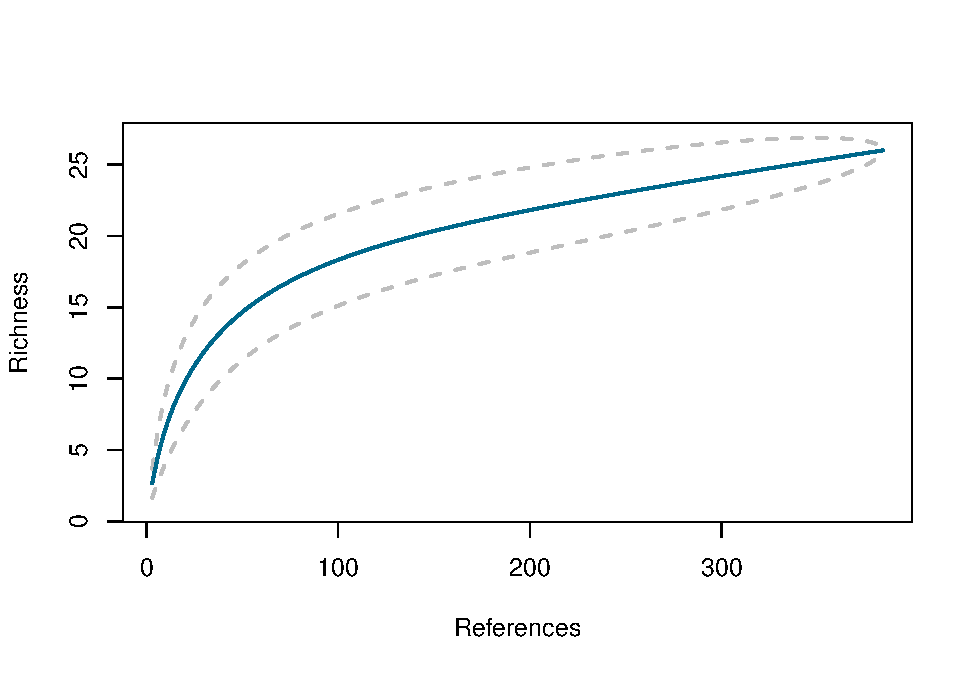
\includegraphics[width=0.8\textwidth]{MA_JJ_files/figure-latex/SACGenera-1.pdf}
	\caption[Sample-based accumulation curve on generic level]{Sample-based accumulation curve of fossil genera per reference. Dashed lines represent the confidence inteval.}
	\label{fig:SACGen}
\end{figure}


\FloatBarrier


%read: Smith and Lyons, 2010 (?) and Smith et al., 2016
%--> body size patterns (see also table 22, general statistics)

%data is bimodal (not normally distributed --> fig. ), still visible in pretty much all subgroups that you could split them into.
%as most animal groups/clades (?) right-skewed = smaller body size more frequent, BUT island species are left-skewed with more larger body sizes! (logtransformed data, skewness: negative for Zanclean, Messinian ??, insular, fossil-insular, but not modern-insular!!)
\subsection{Descriptive statistics}

The histograms indicate that testudinid body size is not normally distributed (Fig. \ref{fig:histAll}), which is supported by QQ-Plots for raw as well as log-transformed data (Fig. \ref{fig:NormDis}).
The body size distribution is moderately right-skewed (Table \ref{tab:stats}), with a higher frequency of smaller body sizes. 
%________________________________________________________________________

\begin{figure}[htbp]
	\centering
	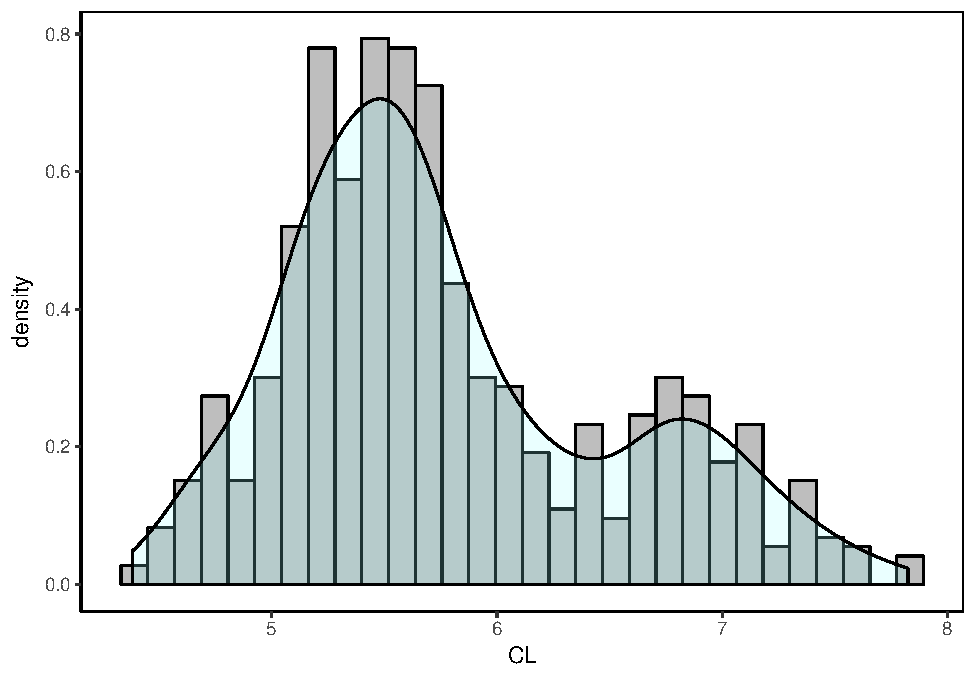
\includegraphics[width=0.8\textwidth]{MA_JJ_files/figure-latex/HistAll-1.pdf}
	\caption[CL distribution]{Body size distribution of complete data set. Bimodally distributed and right-skewed.}
	\label{fig:histAll}
\end{figure}
This pattern is also apparent when splitting the data set into fossil and modern taxa (Fig. \ref{fig:HistFMCI} (a)). Considering insularity, body size distribution is right-skewed for continental taxa, but left-skewed for insular species, meaning larger body size occurs with a higher frequency than smaller body size on islands. Insular taxa are also left-skewed when only considering fossil taxa, but modern insular taxa have a skewness close to 0, indicating a symmetric distribution (Table \ref{tab:stats}).
Kurtosis suggests light tails with no/few outliers (kurtosis < 3) for insular and modern insular species, whereas continental species have a heavy tail (kurtosis > 3; Table \ref{tab:stats}).

\begin{center}
	\begin{figure}[htbp]
		\subfloat[Fossil vs. modern]{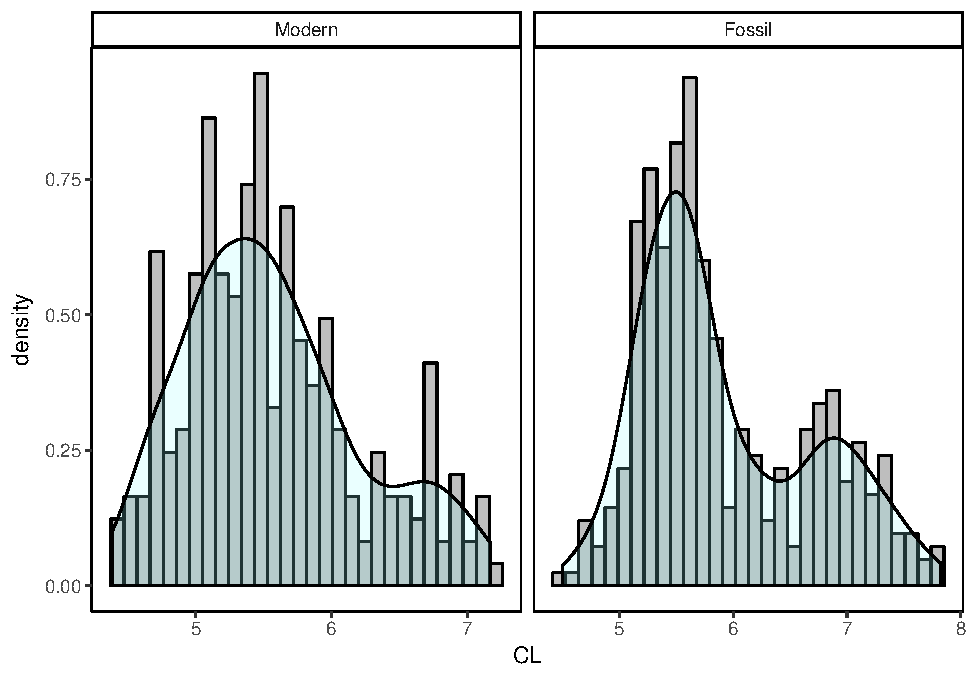
\includegraphics[scale=0.45]{MA_JJ_files/figure-latex/HistFosMo-1.pdf}}
		\subfloat[Continental vs. insular]{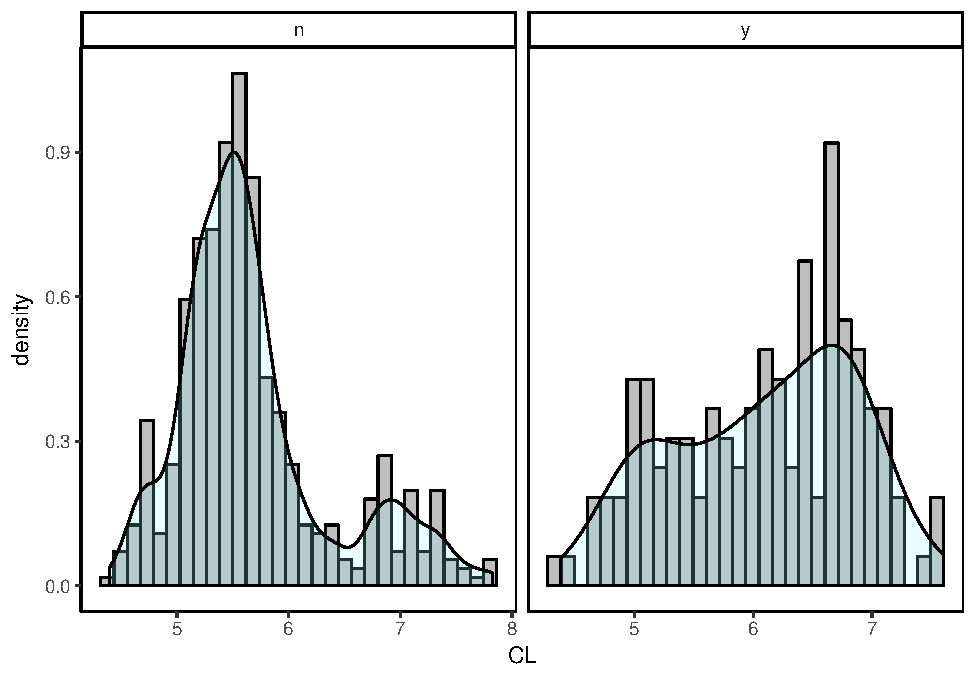
\includegraphics[scale=0.45]{MA_JJ_files/figure-latex/HistCI-1.pdf}}	
		\caption[Fossil vs. modern, continental vs. insular.]{Histograms for fossil vs. modern and continental vs. insular data.}
		\label{fig:HistFMCI}
	\end{figure}
\end{center}

The histograms show a bimodal distribution, wich is also apparent on most sublevels, except for modern insular species (Fig. \ref{fig:HistRest} (a)).
Body size distributions are similar, right-skewed and bimodal, for the four continents and reflect the overall trend (Fig. \ref{fig:HistRest} (b)).




\FloatBarrier

%__________________________



Mean body size differs significantly across time bins (Kruskal Wallis Test, $\chi^2$ = 71.441, P < 0.01; Fig. \ref{fig:boxBins}). 
The multiple comparison test showed that modern median body size is smaller than body size in the Upper Pleistocene. %(Wilcoxon Rank Sum Test, W = 3853.5, P < 0.01 )
There is no difference in body size within the Pleistocene %(Wilcoxon Rank Sum Test, P > 0.05)
and Pleistocene body size does not differ from body size in the Upper Miocene%(Wilcoxon Rank Sum Test, P > 0.05)
. Serravallian body size is smaller than Langhian body size in the Middle Miocene%(Wilcoxon Rank Sum Test, W = 45, P < 0.01)
, but Langhian body size is not different from Lower Miocene body size%(Wilcoxon Rank Sum Test, W = 311, P = 0.06)
.


%__________________________________________________________________________
\begin{figure}[hbtp]
	\centering
	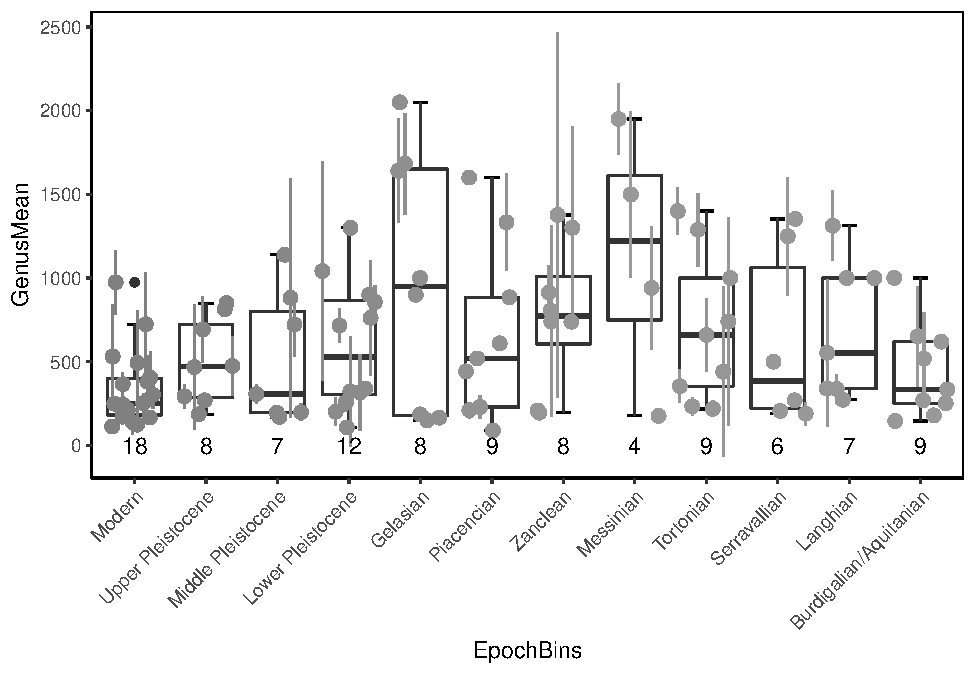
\includegraphics{MA_JJ_files/figure-latex/BPGBins-1.pdf}
	\caption{Boxplots of mean CL per time bin, including mean and sd CL for
		each genus (as pointrange).}
	\label{fig:boxBins}
\end{figure}

%\todo{random sampling necessary?}
% = 71.441, df = 11, p-value = 6.496e-11






%need statistics for boxplot!! kruskal-wallis-test plus post-hoc test (+ bonferroni correction?) or moving mean (faysal?)
%you can kind of see how the median increases and then decreases again
%(compare in order: Modern < Upper Pleistocene etc., do median and variance??)






%__________________________________________________________________________
\begin{center}
	\begin{figure}[htbp]
		\subfloat[Fossil vs. modern]{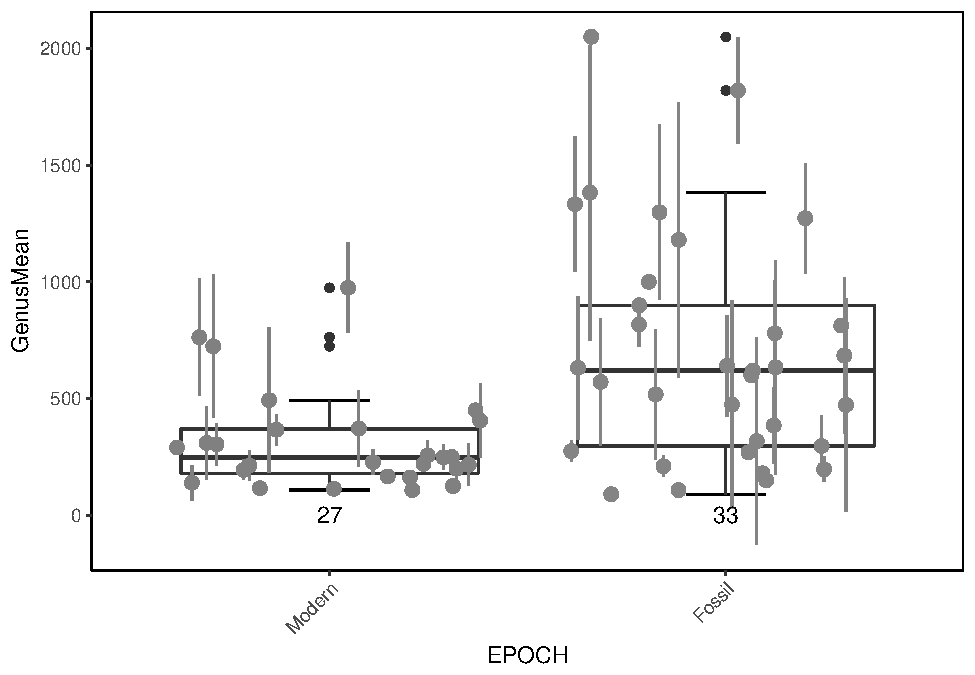
\includegraphics[scale=0.45]{MA_JJ_files/figure-latex/BPMF-1.pdf}}
		\subfloat[Continental vs. insular]{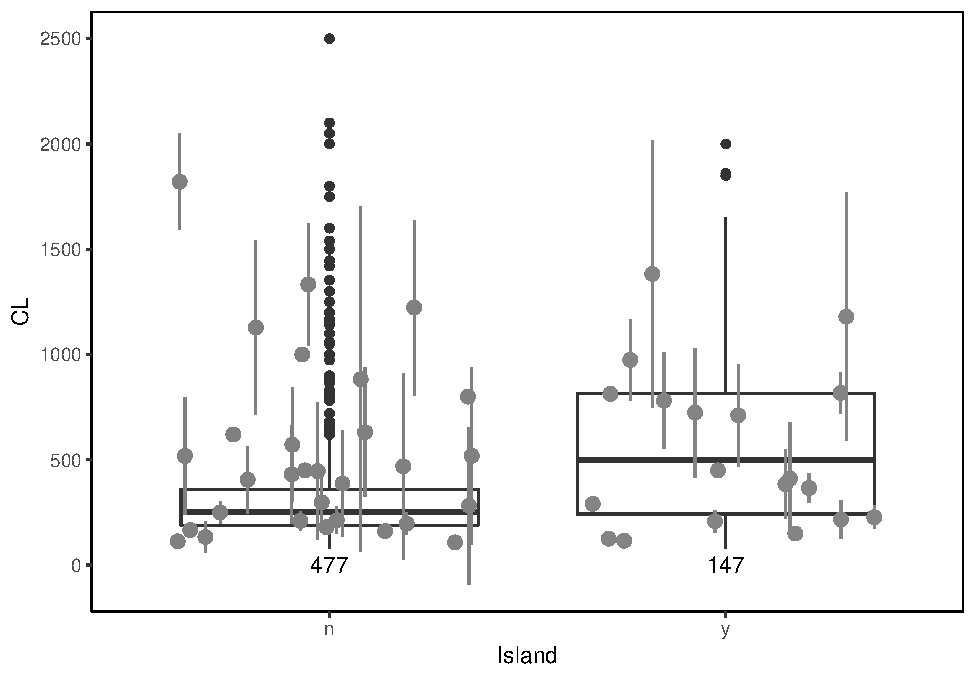
\includegraphics[scale=0.45]{MA_JJ_files/figure-latex/BPCI-1.pdf}}
		\caption{Boxplots of CL split into fossil vs. modern (a) and cotinental vs. insular (b)}
		\label{fig:boxFMCI}
	\end{figure}
\end{center}



Comparison of modern and fossil testudinids showed that modern tortoises are significantly smaller than fossil ones (Wilcoxon Rank Sum Test, W = 22318, P < 0.01; Fig. \ref{fig:boxFMCI}). Furthermore, continental testudinids are significantly smaller than insular taxa (Wilcoxon Rank Sum Test, W = 13854, P < 0.01; Fig. \ref{fig:boxFMCI}).
These results can even be considered in combination: modern continental taxa are smaller than fossil continental taxa (Wilcoxon Rank Sum Test, W = 8046, P < 0.01; Fig. \ref{BoxFoMCI}) and modern insular taxa are smaller than fossil insular taxa (Wilcoxon Rank Sum Test, W = 631.5, P < 0.01; Fig. \ref{BoxFoMCI}))

Finally, body size differs among continents (Kruskal Wallis Test, $\chi^2$ = 34.343, P < 0.01; Fig. \ref{fig:boxCon}). The multiple comparison test showed that African testudinids differ significantly from the other three continents in body size. American testudinid body size is comparable to that of Asia, but differs from those of Africa and Europe. Furthermore, Asian and European testidinids are similar in body size. Since only Europe/Eurasia are well sampled, these relationships could change with further sampling. ??


\begin{figure}[htbp]
	\centering
	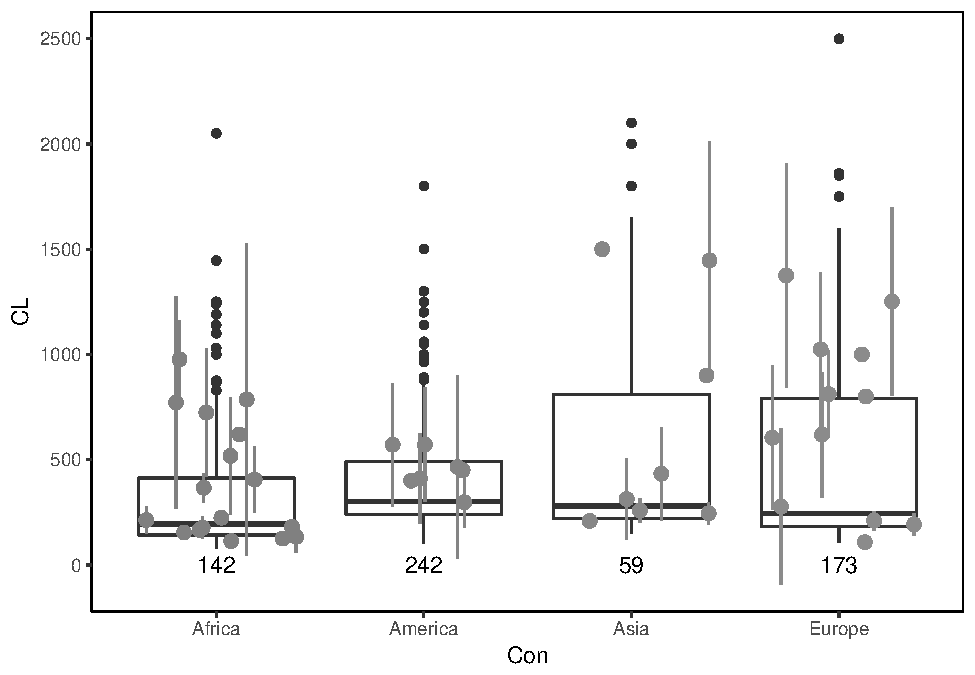
\includegraphics[width=0.75\textwidth]{MA_JJ_files/figure-latex/BPCon-1.pdf}
	\caption{Boxplot: body size on different continents, genera summarised}
	\label{fig:boxCon}
\end{figure}



\FloatBarrier
%__________________________________________________________________________

\subsection{paleoTS analysis}\label{paleots-analysis}




\subsubsection{complete dataset}\label{all-continental-and-insular}

Fitting of the three evolutionary models favoured stasis for the entire data set, although model support was only 51 \% followed by 33 \% support for the unbiased random walk (Fig. \ref{fig:pTSall}, Table \ref{tab:pTSall}). When solely considering continental genera, the best-fitting model was the unbiased random walk, but again not ideally supported with 55 \% (Fig. \ref{fig:pTSC}, Table \ref{tab:pTSCEM}). In contrast, insular genera are best described by stasis, which was very well supported (100 \%; Fig. \ref{fig:pTSI}, Table \ref{tab:pTSIEM})). 


\begin{figure}[H]
	\centering
	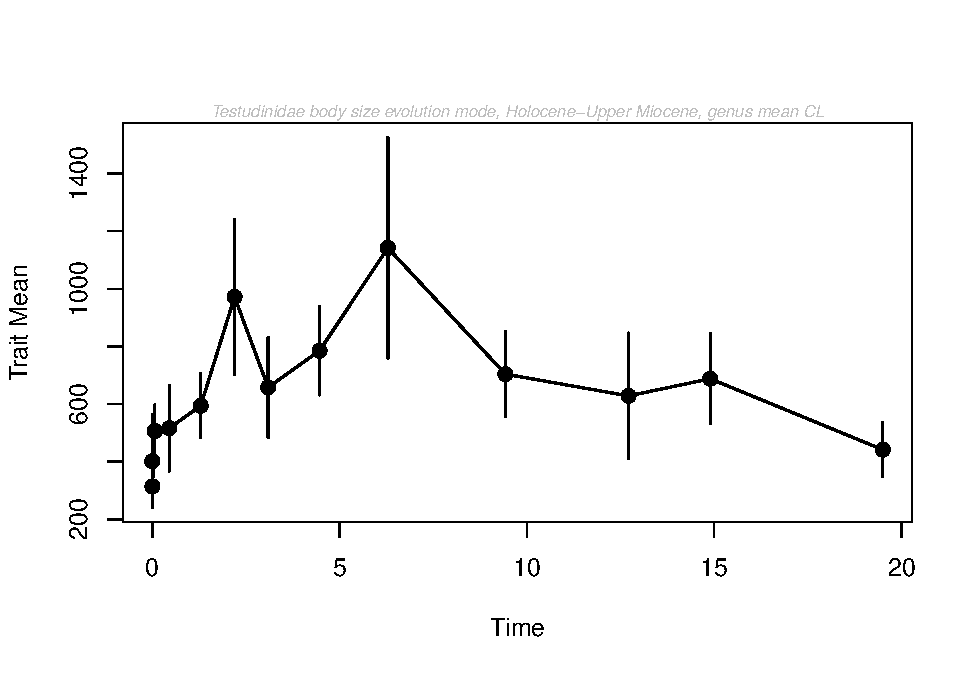
\includegraphics{MA_JJ_files/figure-latex/paleoTSAll-1.pdf}
	\caption{paleoTS plot with genus mean, all}
	\label{fig:pTSall}
\end{figure}

\begin{longtable}[]{@{}lrrrr@{}}
	\caption{Model-fitting results for testudinidae, genera,
		all}
	\label{tab:pTSallEM}\tabularnewline
	\toprule
	& logL & K & AICc & Akaike.wt\tabularnewline
	\midrule
	\endfirsthead
	\toprule
	& logL & K & AICc & Akaike.wt\tabularnewline
	\midrule
	\endhead
	GRW & -81.31790 & 2 & 167.9691 & 0.161\tabularnewline
	URW & -82.05721 & 1 & 166.5144 & 0.332\tabularnewline
	Stasis & -80.16802 & 2 & 165.6694 & 0.507\tabularnewline
	\bottomrule
\end{longtable}

\FloatBarrier
%__________________________________________________________________________

\subsubsection{continental dataset (excluding insular
	species)}\label{continental-excluding-insular-species}


\begin{figure}[H]
	\centering
	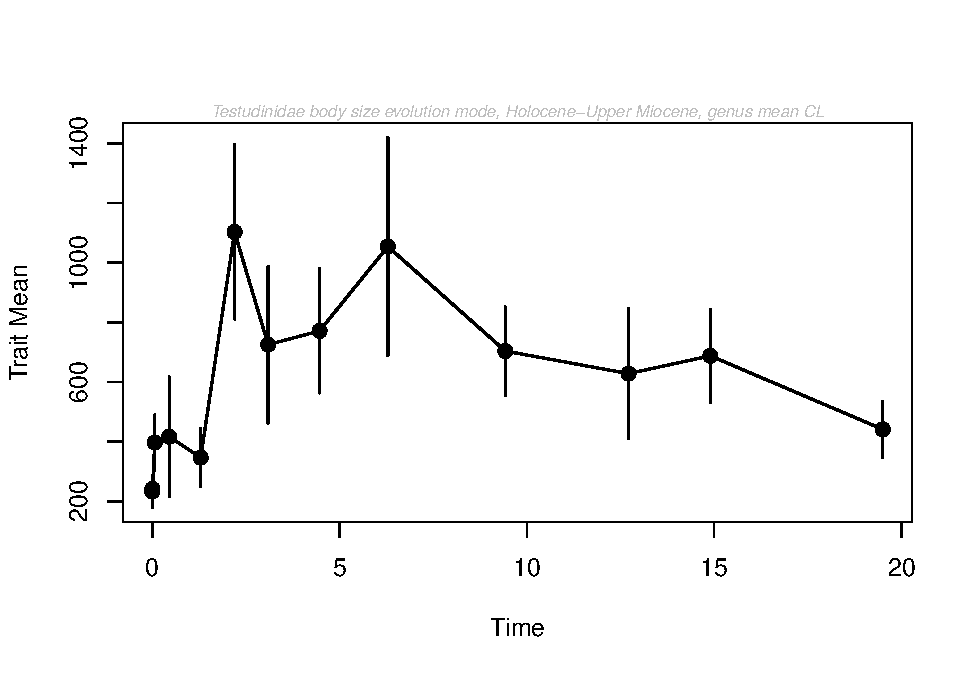
\includegraphics{MA_JJ_files/figure-latex/paleoTSC-1.pdf}
	\caption{paleoTS plot with genus mean, continental}
	\label{fig:pTSC}
\end{figure}

\begin{longtable}[]{@{}lrrrr@{}}
	\caption{Model-fitting results for testudinidae, genera,
		continental}
	\label{tab:pTSCEM}\tabularnewline
	\toprule
	& logL & K & AICc & Akaike.wt\tabularnewline
	\midrule
	\endfirsthead
	\toprule
	& logL & K & AICc & Akaike.wt\tabularnewline
	\midrule
	\endhead
	GRW & -82.26287 & 2 & 169.8591 & 0.300\tabularnewline
	URW & -83.12577 & 1 & 168.6515 & 0.548\tabularnewline
	Stasis & -82.93984 & 2 & 171.2130 & 0.152\tabularnewline
	\bottomrule
\end{longtable}


\FloatBarrier
%__________________________________________________________________________

\subsubsection{insular dataset (excluding
	continental)}\label{insular-excluding-continental}




\begin{figure}[H]
	\centering
	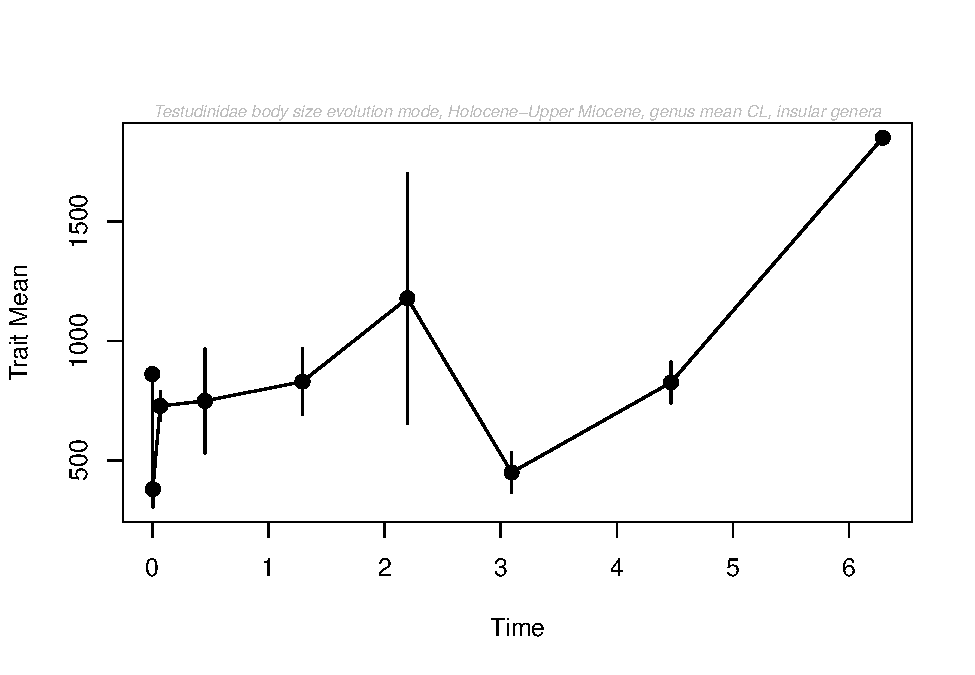
\includegraphics{MA_JJ_files/figure-latex/paleoTSI-1.pdf}
	\caption{paleoTS plot with genus mean, insular}
	\label{fig:pTSI}
\end{figure}

\begin{longtable}[]{@{}lrrrr@{}}
	\caption{Model-fitting results for testudinidae, genera,
		insular}
	\label{tab:pTSIEM}\tabularnewline
	\toprule
	& logL & K & AICc & Akaike.wt\tabularnewline
	\midrule
	\endfirsthead
	\toprule
	& logL & K & AICc & Akaike.wt\tabularnewline
	\midrule
	\endhead
	GRW & -68.57344 & 2 & 143.5469 & 0\tabularnewline
	URW & -75.76576 & 1 & 154.1982 & 0\tabularnewline
	Stasis & -60.41581 & 2 & 127.2316 & 1\tabularnewline
	\bottomrule
\end{longtable}

\FloatBarrier
%__________________________________________________________________________

\subsubsection{per continent}\label{per-continent}

\paragraph{Europe, genera}\label{europe-genera}

When repeating the analysis for European taxa only, all three groups -- complete, continental and insular data -- are best described by stasis with a model support between 92 - 99 \% (Fig. \ref{fig:pTSEu}, \ref{fig:pTSEuC}, \ref{fig:pTSEuI}; Tables \ref{tab:pTSEuEM}, \ref{tab:pTSEuCEM}, \ref{tab:pTSEuIEM}).

\begin{figure}[H]
	\centering
	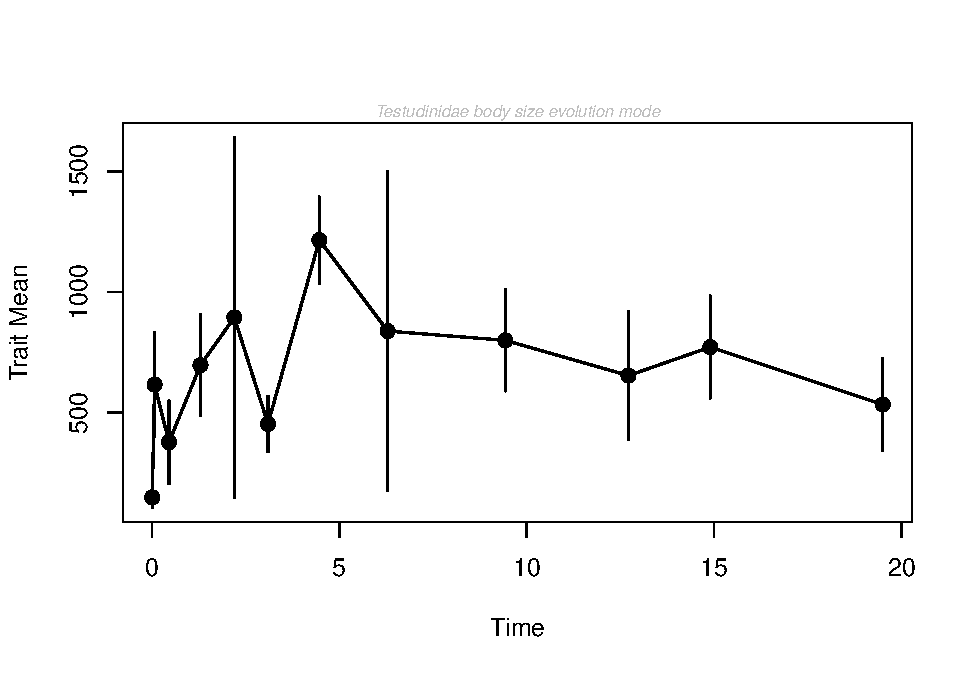
\includegraphics{MA_JJ_files/figure-latex/paleoTSEurope-1.pdf}
	\caption{Genera, Europe}
	\label{fig:pTSEu}
\end{figure}

\begin{longtable}[]{@{}lrrrr@{}}
	\caption{Model-fitting results for testudinidae, genera,
		Europe}
	\label{tab:pTSEuEM}\tabularnewline
	\toprule
	& logL & K & AICc & Akaike.wt\tabularnewline
	\midrule
	\endfirsthead
	\toprule
	& logL & K & AICc & Akaike.wt\tabularnewline
	\midrule
	\endhead
	GRW & -84.14010 & 2 & 173.7802 & 0.006\tabularnewline
	URW & -85.90727 & 1 & 174.2590 & 0.005\tabularnewline
	Stasis & -79.01365 & 2 & 163.5273 & 0.990\tabularnewline
	\bottomrule
\end{longtable}

\FloatBarrier
%__________________________________________________________________________



\paragraph{Eurasia,	genera}\label{eurasia-genera}


For Eurasia, the entire data as well as continental genera are best described by the unbiased random walk, although the model support is weak again. Continental species still have a better support (78 \%; Fig. \ref{fig:pTSEsC}, Table \ref{tab:pTSEsCEM}) than all Eurasian data with only 56 \% (Fig. \ref{fig:pTSEs}, Table \ref{tab:pTSEsEM}). Insular Eurasian species, however, conform to stasis again, although with lower support values (68 \%; Fig. \ref{fig:pTSEsI}, Table \ref{tab:pTSEsIEM}).



\begin{figure}[H]
	\centering
	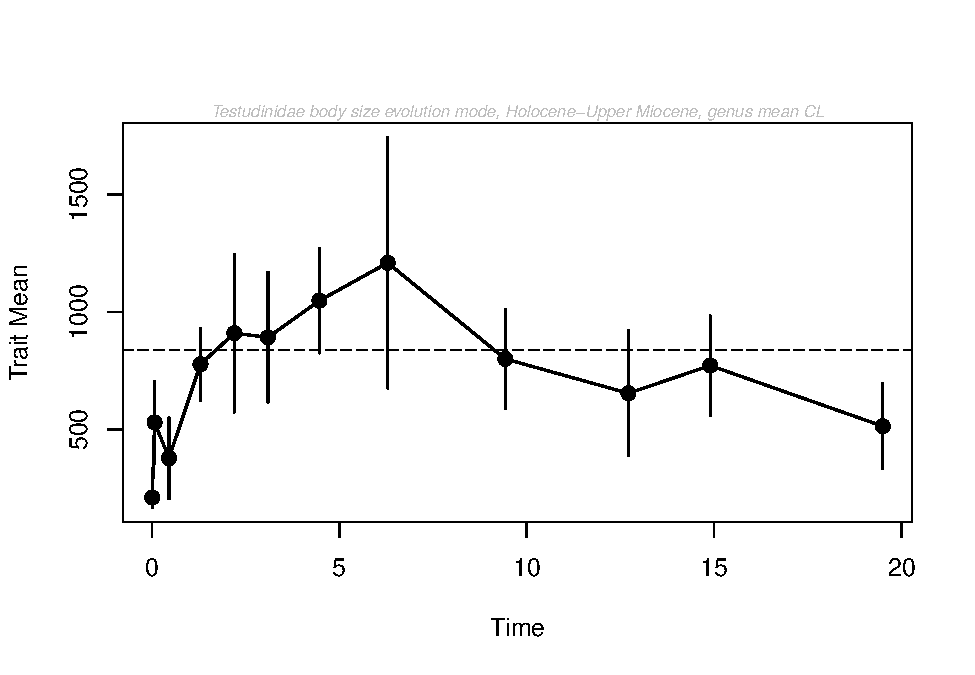
\includegraphics{MA_JJ_files/figure-latex/paleoTSEurasia-1.pdf}
	\caption{paleoTS, genera, Eurasia}
	\label{fig:pTSEs}
\end{figure}

\begin{longtable}[]{@{}lrrrr@{}}
	\caption{Model-fitting results for testudinidae, genera,
		Eurasia}
	\label{tab:pTSEsEM}\tabularnewline
	\toprule
	& logL & K & AICc & Akaike.wt\tabularnewline
	\midrule
	\endfirsthead
	\toprule
	& logL & K & AICc & Akaike.wt\tabularnewline
	\midrule
	\endhead
	GRW & -85.25195 & 2 & 175.8372 & 0.149\tabularnewline
	URW & -85.39072 & 1 & 173.1814 & 0.562\tabularnewline
	Stasis & -84.58890 & 2 & 174.5111 & 0.289\tabularnewline
	\bottomrule
\end{longtable}



\FloatBarrier
%__________________________________________________________________________

